% -- Deckblatt.tex -----------------------------------------------------------
%
%   Gestaltung des Deckblattes der Bedienungsanleitung:  
%   - Einbinden und formatieren der Logos
%   - Bezeichnungen befinden sich in 'Meta.tex'   
% ------------------------------------------------------------------------------

\thispagestyle{empty} % von plain nach empty
\begin{titlepage}
\vspace*{-3cm}% vertikale negative Verschiebung
%%------------------------------------------------------------------------------
%%   Firmenlogo einf�gen
%%------------------------------------------------------------------------------
\begin{figure}[h]
\centering

\includegraphics[width=0.25\textwidth]{schlizbaeda.png}
\end{figure}

\begin{center}
\LARGE{\textbf{\Dokumentart}}\\[1.5ex] 
\Large{\Bezeichnung}\\[4ex]
%%------------------------------------------------------------------------------
%%   Titel der Bedienungsanleitung
%%------------------------------------------------------------------------------
\noindent\rule[1ex]{\textwidth}{3pt} % vertikaler Strich
%\huge{\textbf{\titel}}\\[1.5ex]      % TITEL DER ARBEIT
\textbf{\titel}\\[1.5ex]              % TITEL DER ARBEIT (lange �berschrift)
\noindent\rule[1ex]{\textwidth}{3pt} 
%\LARGE{\textbf{\untertitel}}\\[6ex]
%\LARGE{\textbf{\art}}\\[1.5ex]
%\Large{im Fachgebiet \fachgebiet}
\\[2ex]

\normalsize
%%------------------------------------------------------------------------------
%%   Bild
%%------------------------------------------------------------------------------
\textbf{\\}
\begin{figure}[h]
\centering
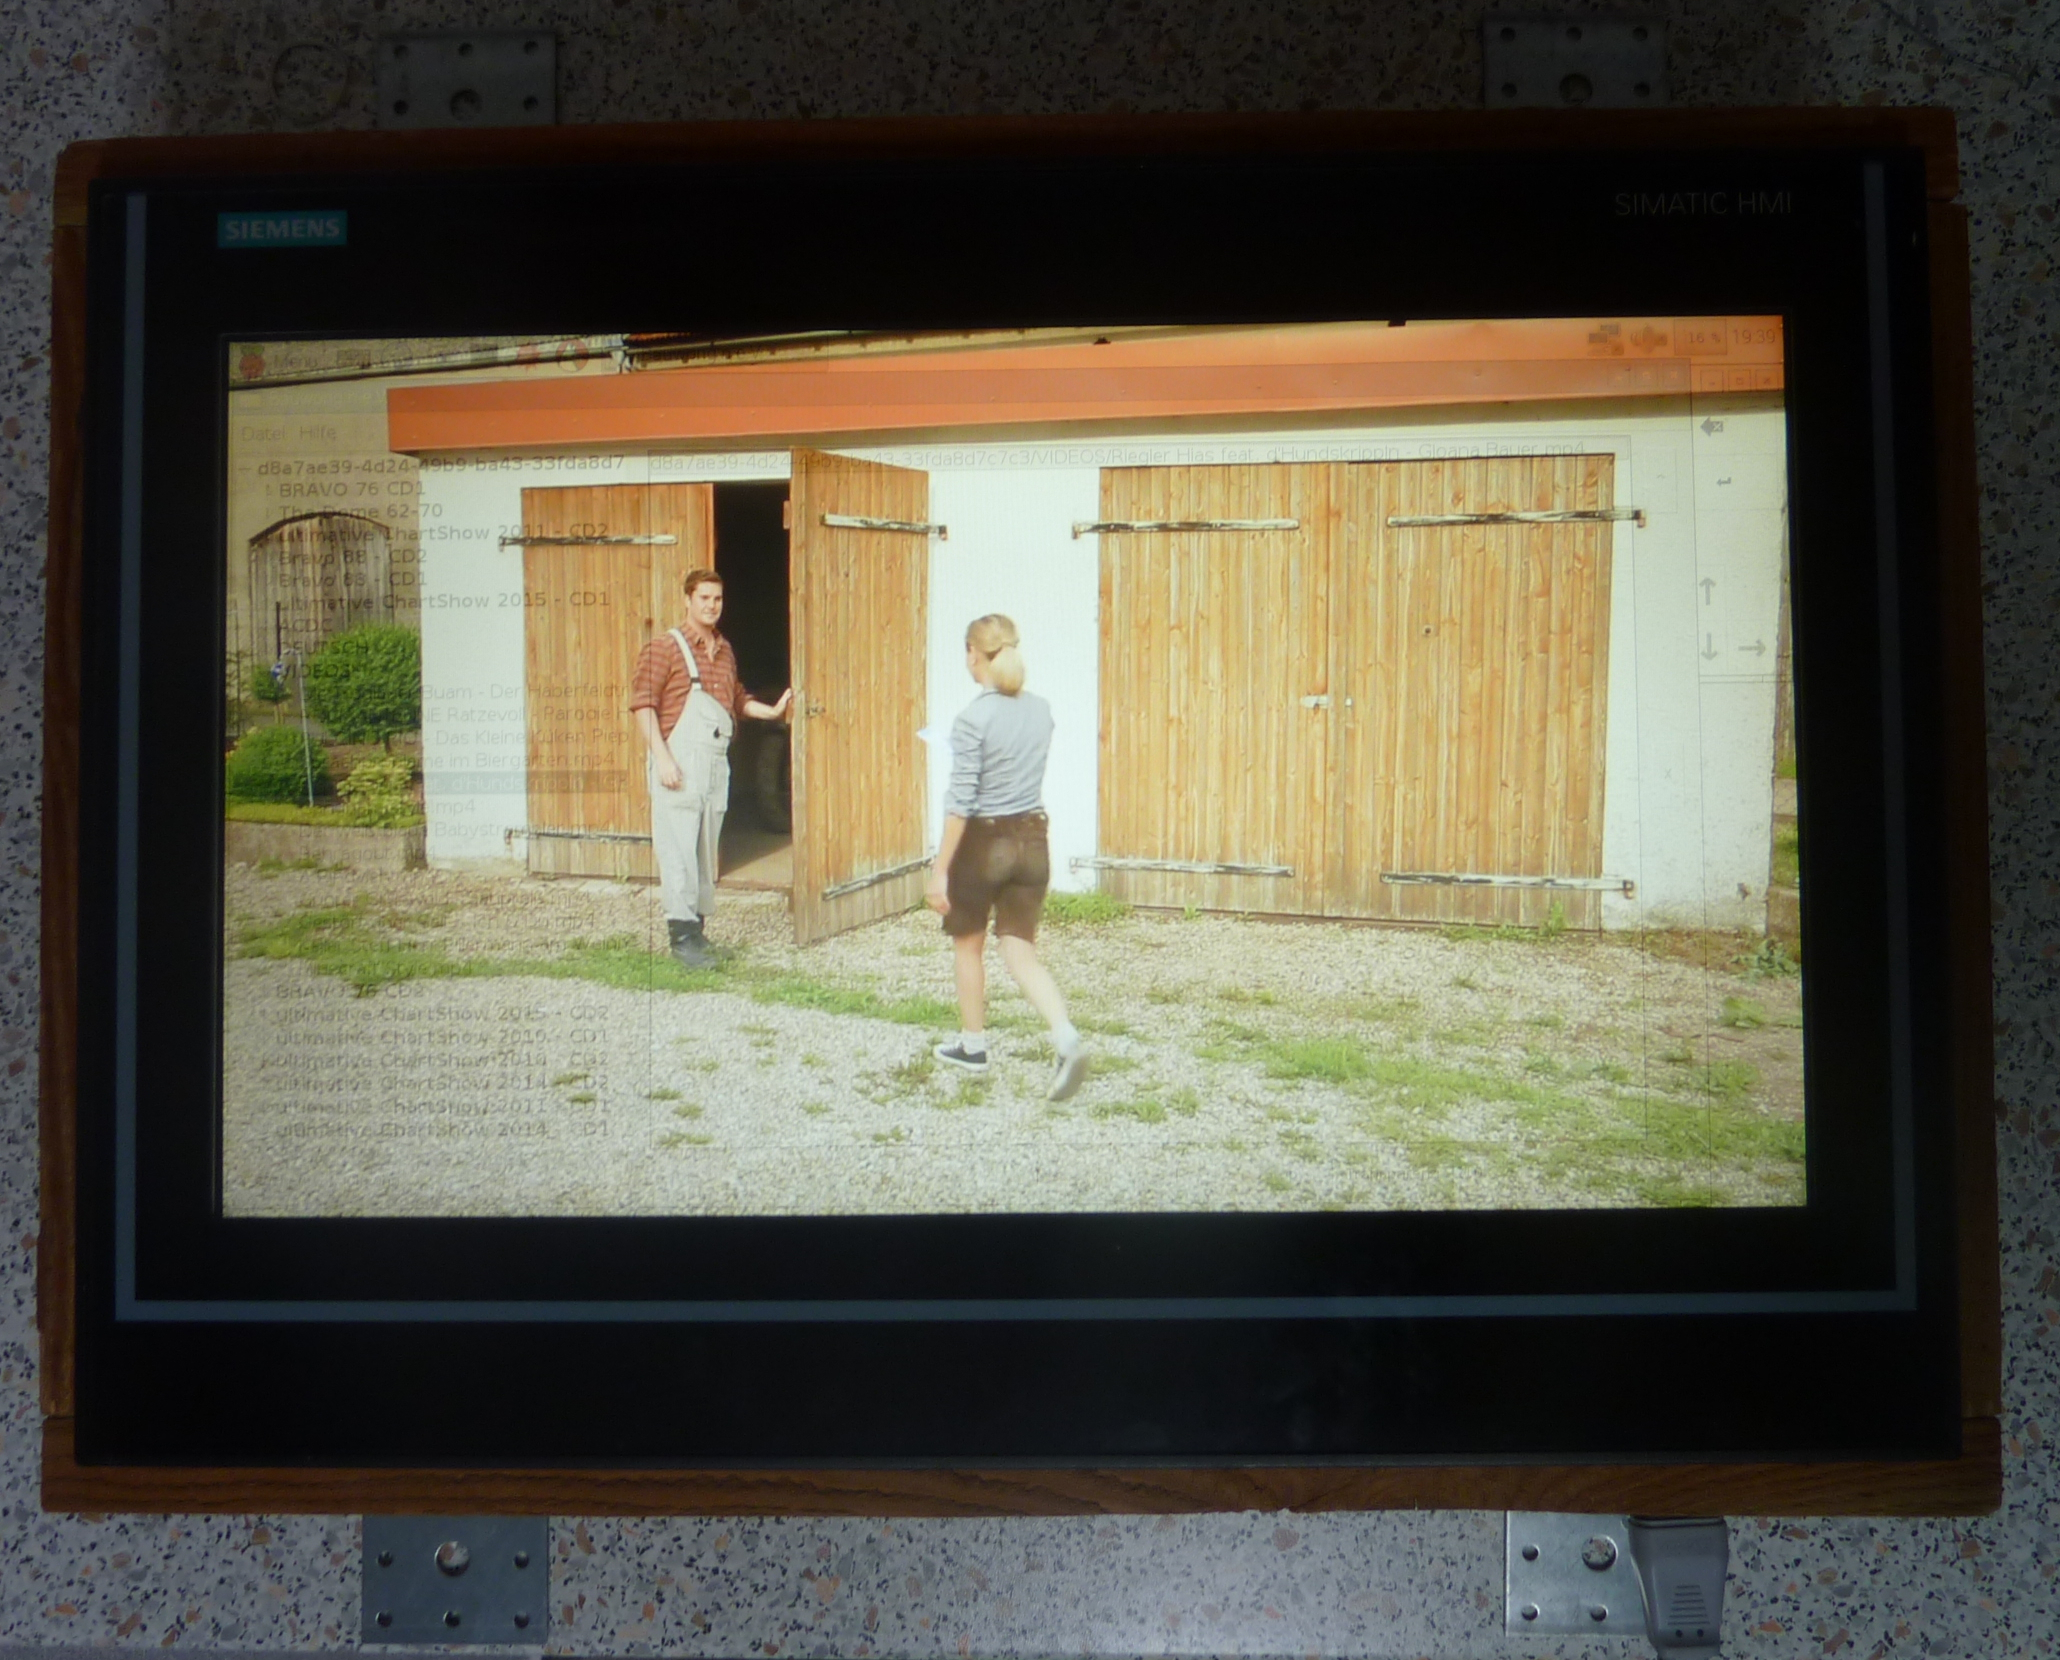
\includegraphics[width=12cm]{Titelbild.jpg}
\end{figure}

%%------------------------------------------------------------------------------
%%   GNU-Logo, Copyrighthinweis, GPLv3-Logo
%%------------------------------------------------------------------------------
\begin{tabular}{lllr}\\
\hline
% --- Zeile mit de offiziellen Logo der Free Software Foundation:
\parbox[c][50px]{0.10\textwidth}{
\includegraphics[height=35px]{GNU.png}} & \parbox[c]{0.40\textwidth}{GNU General Public License v3\\ \copyright\ 2016 - 2017 by \autor}  & \parbox[c]{0.15\textwidth}{Datum:\\18.08.2017} & \parbox[c][50px]{0.20\textwidth}{
\includegraphics[height=35px]{GPLv3.png}}\\
\hline
\end{tabular}

\end{center}

\textbf{}\\
Die Abbildung auf dem Display stammt aus dem Video zu folgendem Musikst�ck:\\
\texttt{\textbf{Riegler Hias feat. d' Hundskrippln} \textit{Gloana Bauer}} bei 2:42\\
\url{https://www.hundskrippln.de/#filme} %-- 2:42

\end{titlepage}



